\documentclass{sig-alternate}
\usepackage{graphicx}
\usepackage{url}
\usepackage{paralist}
\usepackage{listings}

% \DeclareUnicodeCharacter{B1}{\pm}
%% LANGUAGE      Markup definitions
\def\lstxml{
  \lstset{language=XML,
    keywordstyle=\ttfamily,
    identifierstyle=\ttfamily\bfseries, 
    % commentstyle=\color{Brown},
    stringstyle=\ttfamily,
    showstringspaces=false,
    columns=[l]flexible, %% , basewidth={0.5em,0.4em}
    escapeinside={(@*}{*@)},
    morekeywords={encoding,
      mrow,math,mfrac,mi,msqrt,mo,mn,span,nobr,img}
  }
}

\def\lstjs{
  \lstset{language=Java,
    keywordstyle=\ttfamily,
    identifierstyle=\ttfamily\bfseries, 
    % commentstyle=\color{Brown},
    stringstyle=\ttfamily,
    showstringspaces=false,
    columns=[l]flexible, %% , basewidth={0.5em,0.4em}
    morekeywords={cvox,Api,Math,defineRule}
  }
}

\def\lsttex{
  \lstset{language={[LaTeX]TeX},
    texcsstyle=*\bfseries,
    keywordstyle=\ttfamily,
    identifierstyle=\ttfamily\bfseries, 
    % commentstyle=\color{Brown},
    stringstyle=\ttfamily,
    showstringspaces=false,
    columns=[l]flexible, %% , basewidth={0.5em,0.4em}
    moretexcs=intertext,
    morekeywords={sum,Sigma}
  }
}

\newcommand\ednote[1]{\typeout{There is still a note!!!}%
  {\bf EDNOTE: #1}}

\newcommand\edbf[1]{\typeout{There is still an editor's note!!!}%
  \textbf{EDNOTE: #1}}


\begin{document}
\title{Accessibility to Scientific Material:\\ The Case of Speaking Math}
\numberofauthors{2} %  in this sample file, there are a *total*

\author{
% You can go ahead and credit any number of authors here,
% e.g. one 'row of three' or two rows (consisting of one row of three
% and a second row of one, two or three).
%
% The command \alignauthor (no curly braces needed) should
% precede each author name, affiliation/snail-mail address and
% e-mail address. Additionally, tag each line of
% affiliation/address with \affaddr, and tag the
% e-mail address with \email.
%
% 1st. author
  \alignauthor Volker Sorge\titlenote{This work was done while the author spent a
    sabbatical at Google,
    Inc., Mountain View, CA, USA.}\\
  \affaddr{School of Computer Science}\\
  \affaddr{The University of Birmingham, UK}\\
  \email{V.Sorge@cs.bham.ac.uk}
% 2nd. author
\alignauthor
Charles Chen, T.V. Raman, David Tseng\\
       \affaddr{Google, Inc.}\\
       \affaddr{Mountain View, CA, USA}\\
       \email{\{clchen|raman|dtseng\}@google.com}
}


\maketitle 
\begin{abstract} 
  As the traditional methods of publishing and teaching in the
  STEM subjects are being progressively replaced by the provision
  of web-based content, ensuring full accessibility to this
  material for visually impaired users is of paramount importance
  for inclusive education. The text to speech translation of
  content for which well defined markup languages exists such as
  mathematics is a non-trivial problem. In this paper we present
  our efforts of making the speech translation of mathematical
  formulas a first class citizen in a general screen reader. We
  describe the ChromeVox screen reader and demonstrate how its
  features enable us to provide text to speech translation for
  web-based mathematical content. These features allow us to
  translate formulas given in a variety of formats into uniform
  spoken utterances exploiting ChromeVox's ability to handle
  alternative representations of DOM elements. This also allows
  us to customise aural rendering of mathematics both by using
  semantically enriched representations and employing flexible
  and adaptable speech rules. To further aid understanding of the
  math we exploit ChromeVox's idea of letting users engage with
  content on different levels of granularity to enable
  interactive exploration of complex mathematical formulas.
\end{abstract}
\category{H.5.2}{User Interfaces}{Voice I/O}
%A category including the fourth, optional field follows...
\category{H.5.4}{Hypertext}{Navigation, User Issues}

% \terms{}

\keywords{scree reader, mathematics, ChromeVox}

\section{Introduction}\label{sec:intro} As we move away from the traditional
methods of publishing and teaching to the provision of web-based content, more
and more scientific literature and teaching material in the STEM subjects
becomes available online. This material can range from traditional articles
containing mathematical formulas and scientific diagrams to highly interactive
webpages often exploiting novel media formats such as dynamic diagrams or
simulations. Ensuring full accessibility to this material for users that rely
primarily on voice output from their computer becomes a challenging
problem. Already the text to speech translation of fairly conventional
scientific content like mathematical formulae, which contain rich structure and
for which a well defined markup language exists, is non-trivial.


\ednote{Some related work here.}

In this paper we report on our effort to integrate the basic support
for voicing mathematical content on the web into the ChromeVox screen
reader. 


% A major prerequisite for the comprehension of scientific literature is for a
% reader to be able to engage with the content.

% this is not as straight forward for a 


As an example we consider the quadratic formula:
\begin{equation}
  \label{eq:quadratic}
  x=\frac{-b \pm \sqrt {b^2-4ac}}{2a}
\end{equation}


We shall present some of the main challenges to making maths
on the web accessible, where it is given in a variety of ways and
formats. We shall outline the rule based approach we have pursued and
how it fits with ChromeVox's philosophy to enable users to explore
content at different levels of granularity. It has led to an
implementation of a flexible speech rule engine that allows to
customise the reading experience along several axes and that also
provides an API for easy adaptation to specialised content by users
and web site authors.

\section{Mathematics on the Web}
\label{sec:math}

Mathematical formulas on webpages can be represented in their own specialised
markup language, MathML~\cite{MathML3}. But although MathML is officially part
of the HTML5 standard~\cite{HTML5}, not all major browsers also implement MathML
rendering, hence support displaying formulas included in pure MathML on web
pages is sketchy. Consequently in reality mathematics on the web comes in a
variety of flavours. One can identify predominant three ways in which
mathematical content is currently given on the web:
\begin{enumerate}
\item Pure MathML markup: this relies on the user viewing the
  page with a browser that renders MathML.
\item Rendered with MathJax: the webpage author ensures that mathematical
  content is rendered client-side independent of the user's browser by including
  the third party MathJax library in the page. Formulas can be given in several
  different markup languages.  and relying on the third party that renders
  mathematical content client side.
\item Pre-rendered images: Content is ensured to display correctly, by including
  images of formulas in the webpage. The original markup from which the content
  was originally rendered is often given in an attribute of the image tag.
\end{enumerate}

In order to enable access to the majority of mathematics that can be found on
the web today, one hasd to provide text-to-speech support for all of the above
formats, which we shall briefly sketch the remainder of this section.

\subsection{MathML}
\label{sec:mathml}

MathML is a specialised markup language that was developed with the expressive
purpose of representing mathematics. Ordinarily it comes in two flavours:
presentation MathML and content MathML. The former is a markup language geared
towards adequately displaying mathematical formulas thus playing a role of web
documents similar to the one of {\LaTeX} for printed documents.  Contrary,
content MathML aims to serve also as a meaningful exchange format between
mathematical software systems by providing markup that allows to express
semantic meaning of mathematical expressions. As there is still very little
support for content MathML we concentrate here on presentation MathML only.
  
\begin{figure}[t!]
  \begin{center}
    \leavevmode
    \lstxml\small
\begin{lstlisting}
<math xmlns="http://www.w3.org/1998/Math/MathML">
  <mstyle displaystyle="true">
    <mi>x</mi>
    <mo>=</mo>
    <mfrac>
      <mrow>
        <mo>&#x2212;</mo>
        <mi>b</mi>
        <mo>&#x00B1;</mo>
        <msqrt>
          <msup>
            <mi>b</mi>
            <mn>2</mn>
          </msup>
          <mo>&#x2212;</mo>
          <mn>4</mn>
          <mi>a</mi>
          <mi>c</mi>
        </msqrt>
      </mrow>
      <mrow>
        <mn>2</mn>
        <mi>a</mi>
      </mrow>
    </mfrac>
  </mstyle>
</math>
\end{lstlisting}
    \caption{MathML representations of~\ref{eq:quadratic}.}
    \label{fig:quadratic-mml}
  \end{center}
\end{figure}

Presentation MathML provides markup for the most common layout elements
encountered in mathematics, such as sub- and superscripts, fractions, square
roots etc.  In addition it provides markup to define mathematics specific styles
or spacing, as well as specialised attributes such as for fonts, accents, etc.
Fig.~\ref{fig:quadratic-mml} presents our example the quadratic
formula~\ref{eq:quadratic} in MathML markup. Here the tags \texttt{mi},
\texttt{mn}, and \texttt{mo} markup identifiers, number, and operators,
respectively, while layout elements fraction, square root and superscript are
enclosed in the elements \texttt{mfrac}, \texttt{msqrt}, and \texttt{msup}. The
\texttt{mrow} tag allows the horizontal combination of a string of elements, in
case they need to be combined to a single node as in the case of the two
arguments for the fraction tag \texttt{mfrac}.

MathML is part of the specification for the HTML5 standard~\cite{HTML5}, where
it lives in its own namespace. By extension it is also part of the ePub3
standard~\cite{epub3} and consequently one can anticipate that future
implementations of these standards with include native rendering of MathML
content. However, in the current situation only few browsers and epub readers
support MathML and rendering is either achieved by specialist browser plugins or
by third party libraries.


\subsection{MathJax Rendering}
\label{sec:mathjax}

MathJax is a javascript display engine~\cite{MathJax2.2} that consistently
renders mathematical expressions in all browsers. It handles a number of input
formats and translates them into simple HTML markup that visually renders a math
expression in a browser, regardless of whether it supports MathML.  Thus the
basic goal is to shift control on whether and how formulas are displayed to the
content author, by allowing them to include javascript in webpages that calls
MathJax via a content distribution network to enable client side rendering of
math expressions.

\begin{figure*}[b!]
  \begin{center}
    \leavevmode
    \lstxml\small
    \lstinputlisting{mathjax.xml}
    \caption{MathJax representations of~\ref{eq:quadratic} from
      \protect\url{en.wikipedia.org/wiki/Quadratic_equation}.}
    \label{fig:quadratic-mj}
  \end{center}
\end{figure*}

An authors can then include formulas directly into a webpage either as MathML
markup or as {\LaTeX} or AsciiMath~\cite{asciimath}. During the rendering
process MathJax replaces this markup with HTML elements that explicitly specify
vertical and horizontal spacing, drawing of lines and special elements such as
radices, and placement of character in webfonts.  This has not only the
advantage that the generated markup is portable between browsers, but also that
expressions rendered with MathJax are fully scalable.  But since the rendered
expressions that MathJax injects into the DOM is primarily aimed at visual
display, it is a less straigtforward translation of the mathematical expression
it models.

As an example Fig.~\ref{fig:quadratic-mj} shows part of the MathJax markup for
equation~\ref{eq:quadratic}. While it is clearly more cluttered than its MathML
counterpart in Fig.~\ref{fig:quadratic-mml}, there are nevertheless some obvious
resemblances. The expression effectively consists of two types of \texttt{span}
elements:
\begin{inparaenum}[(a)]
\item Those with a single style attribute that are exclusively display elements.
\item Those with a additional class attributes and id that generally mirror the
  composition of the corresponding MathML expression.
\end{inparaenum}
As we can observe in our example, the latter type of elements maintains the
structure of the MathML expression, and this regardless of the original source
of the formula. Indeed MathJax always maintains an internal MathML
representation of a mathematical formula, even if translated from {\LaTeX} or
AsciiMath, a fact that we shall exploit in Sec.~\ref{sec:alternative}.


\subsection{Hidden Markup}\label{sec:images}

Traditionally mathematical formulas would be embedded into web content using
images generated from documents that were previously generated with systems
specialising on rendering mathematics, for example, {\LaTeX}. And despite the
obvious drawbacks of having content in images, such as lack of scalability, this
method is still an option that is chosen by many major web sites containing
mathematical content (e.g., Wikipedia~\cite{wikipedia},
MathWorld~\cite{mathworld}), to provide content consistently at reliable
performance, independent of third party libraries.  While the mathematics given
in image form is effectively inaccessible, the original source from which a
formula has been generated is often given in form of alternative text attribute
of the image tag.  For instance, in the case of Wikipedia, most of the
mathematics images have alternative text provided in \LaTeX, whereas Mathworld
contains AsciiMath markup.  The case of our example is given in
Fig.~\ref{fig:quadratic-img} the quadratic equation is loaded as a PNG images,
while the hidden markup is given in the original \LaTeX.

This form of hidden markup can then be displayed in
text-only browers or used for copy-and-paste operations. 
In ChromeVox we exploit hidden markup as well, to ensure a consistent
screenreading experience of all mathematical content on the web.  In particular,
we rely on the MathJax library to translate hidden markup into a MathML
representation that we can speak instead. We describe in detail the treatment of
alternative representations in Sec.~\ref{sec:alternative}.


\begin{figure*}[t!]
  \begin{center}
    \leavevmode
    \lstxml\small
\begin{lstlisting}
<img class="tex" 
      alt="x=\frac{-b \pm \sqrt {b^2-4ac}}{2a}" 
      src="//upload.wikimedia.org/math/3/c/a/3ca857f705daba6b9e6e6d3ccad7990f.png" />
\end{lstlisting}
\caption{Image markup for~\ref{eq:quadratic} from 
  \protect\url{en.wikipedia.org/wiki/Quadratic_equation}.}
\label{fig:quadratic-img}
  \end{center}
\end{figure*}

\verb+x=\frac{-b \pm \sqrt {b^2-4ac}}{2a}+

\section{ChromeVox}
\label{sec:chromevox}


\subsection{Axes 1: Granularities}
\label{sec:ax1}


\begin{figure}[h!]
  \begin{center}
    \leavevmode
    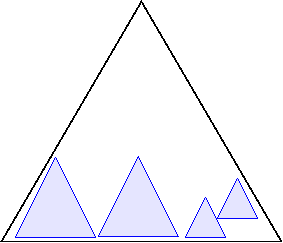
\includegraphics[width=.4\columnwidth]{images/granularity1}
    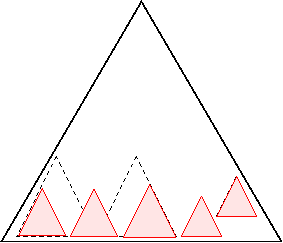
\includegraphics[width=.4\columnwidth]{images/granularity2}
    \caption{Schematic depiction of granularities.}
    \label{fig:granularity}
  \end{center}
\end{figure}

\subsection{Axes 2: Walking}
\label{sec:ax2}


\begin{figure}[h!]
  \begin{center}
    \leavevmode
    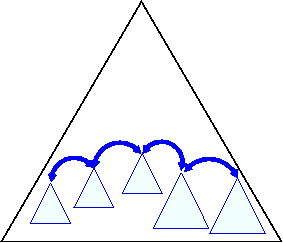
\includegraphics[width=.4\columnwidth]{images/walker1}
    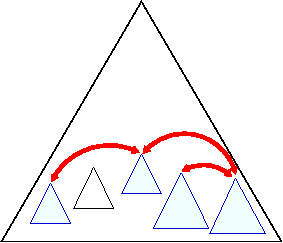
\includegraphics[width=.4\columnwidth]{images/walker2}
    \caption{Schematic depiction of different walkers.}
    \label{fig:walkers}
  \end{center}
\end{figure}

\subsection{Axes 3: Speech Translation}
\label{sec:ax1}



\subsection{Axes 4: Representation}
\label{sec:ax1}


\begin{figure}[h!]
  \begin{center}
    \leavevmode
    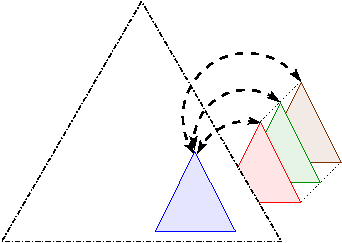
\includegraphics[width=.5\columnwidth]{images/substructure1}
    \caption{Schematic depiction of alternative represenatations.}
    \label{fig:walkers}
  \end{center}
\end{figure}

\section{Speaking Mathematics}
\label{sec:translate}

\section{Alternative Representations}
\label{sec:alternative}

\section{Engaging with Content}
\label{sec:explore}


\section{Conclusions}
\label{sec:conc}


\bibliographystyle{plain} \bibliography{www_2014}

\end{document}
